\documentclass{standalone}
\usepackage{tikz}
\begin{document}
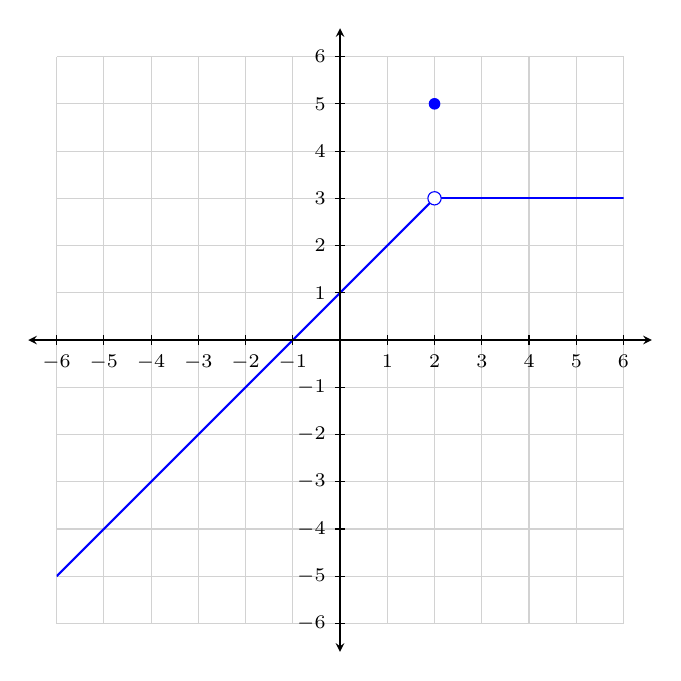
\begin{tikzpicture}[>=stealth, scale=0.6]
  % Graph of y = g(x): removable discontinuity at x = 2
  %   g(x) = x + 1 for x < 2, g(x) = 3 for x > 2
  %   open circle at (2,3) (limit value), filled dot at (2,5) = g(2)
  % Light gray grid
  \draw[gray!35, thin] (-6,-6) grid (6,6);
  % Function graph (clipped to the grid region)
  \begin{scope}
    \clip (-6,-6) rectangle (6,6);
    \draw[blue, thick] (-6,-5) -- (2,3);   % y = x + 1
    \draw[blue, thick] (2,3) -- (6,3);     % y = 3
  \end{scope}
  % Axes with arrows on both ends
  \draw[<->] (-6.6,0) -- (6.6,0);
  \draw[<->] (0,-6.6) -- (0,6.6);
  % x-axis tick labels
  \foreach \x in {-6,-5,-4,-3,-2,-1,1,2,3,4,5,6} {
    \draw (\x,0.1) -- (\x,-0.1) node[below, font=\scriptsize] {$\x$};
  }
  % y-axis tick labels
  \foreach \y in {-6,-5,-4,-3,-2,-1,1,2,3,4,5,6} {
    \draw (0.1,\y) -- (-0.1,\y) node[left, font=\scriptsize] {$\y$};
  }
  % Open circle at (2,3): limit of g(x) as x -> 2
  \draw[fill=white, draw=blue] (2,3) circle (4pt);
  % Filled dot at (2,5): g(2) = 5
  \fill[blue] (2,5) circle (3.5pt);
\end{tikzpicture}
\end{document}
